%%%%%%%%%%%%%%%%%%%%%%%%%%%%%%%%%
\chapter{Results with 13 TeV data}
\label{ch:results13}
%%%%%%%%%%%%%%%%%%%%%%%%%%%%%%%%%

In this chapter, the final results of the analysis performed with 13\TeV data and focused on the search for a heavy resonances decaying into a pair of vector bosons (WW/WZ)
in the $\ell\nu\qqbar$ final state, are presented and discussed.
As for the analysis conducted with 8\TeV data described in the previous chapter, the final \mWV spectrum observed in data is used to check for the presence of a new resonance.
No bins with an excess with significance larger than three standard deviations are observed and upper limits are set on the production cross section of such resonances under a variety of signal benchmarks by combining all the event categories.

%%%%%%%%%%%%%%%%%%%%%%%%%%%%%%%%%
\section{Final $\mWV$ distribution}
%%%%%%%%%%%%%%%%%%%%%%%%%%%%%%%%%

The final \mWV spectra observed in data and for the background predicted with the $\alpha$ ratio method (Section~\ref{sec:alpha}) for all event categories are shown in Fig.~\ref{fig:mWV-final}.
The observed data and the predicted background are found to well agree. The highest mass events are at \mWV = 2.95 and 3.15\TeV for the muon and electron category, respectively.

\begin{figure}[!htb]
\centering
\subfigure[]{\label{fig:mWV-final_a}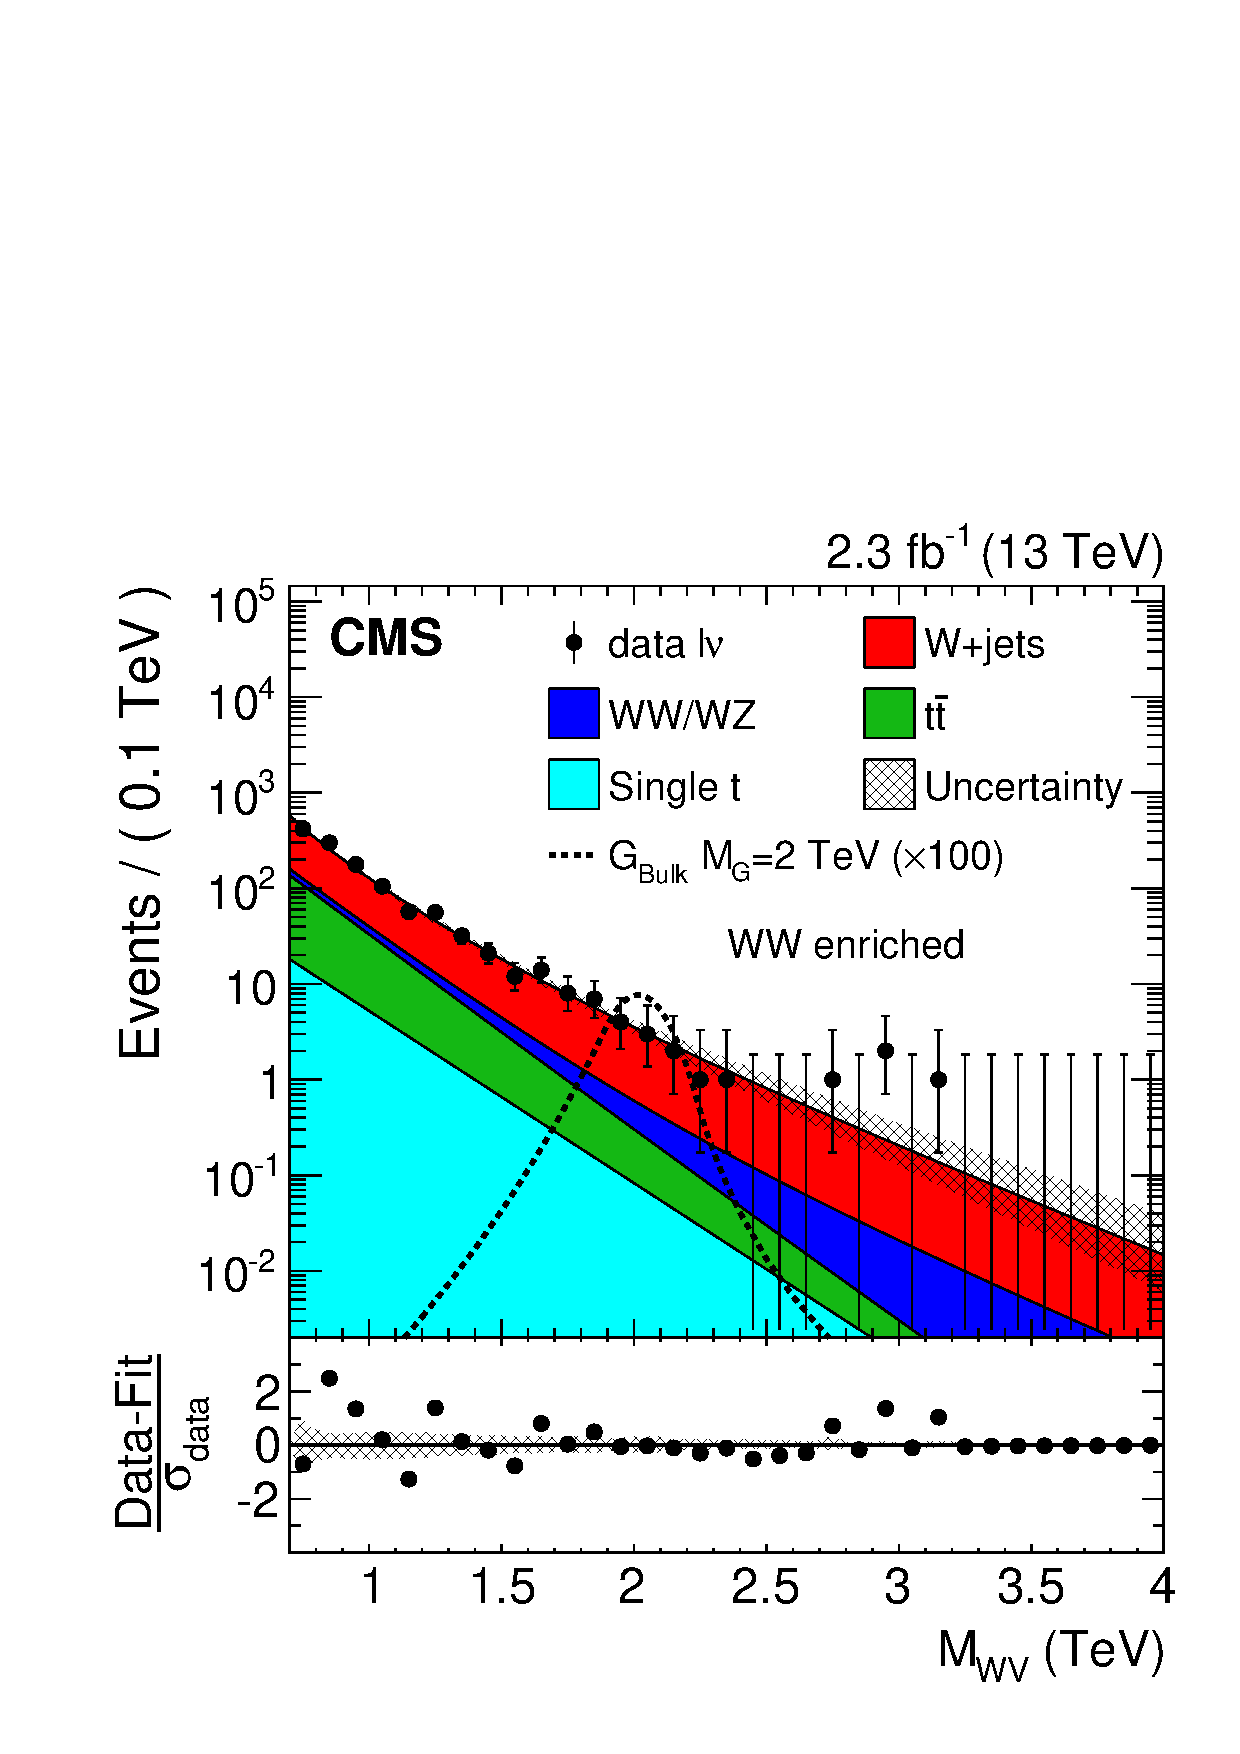
\includegraphics[width=0.45\textwidth]{\chten/HPW_mlvj_fitting-em-check_workspace_for_limit__with_pull_log.pdf}}
\subfigure[]{\label{fig:mWV-final_b}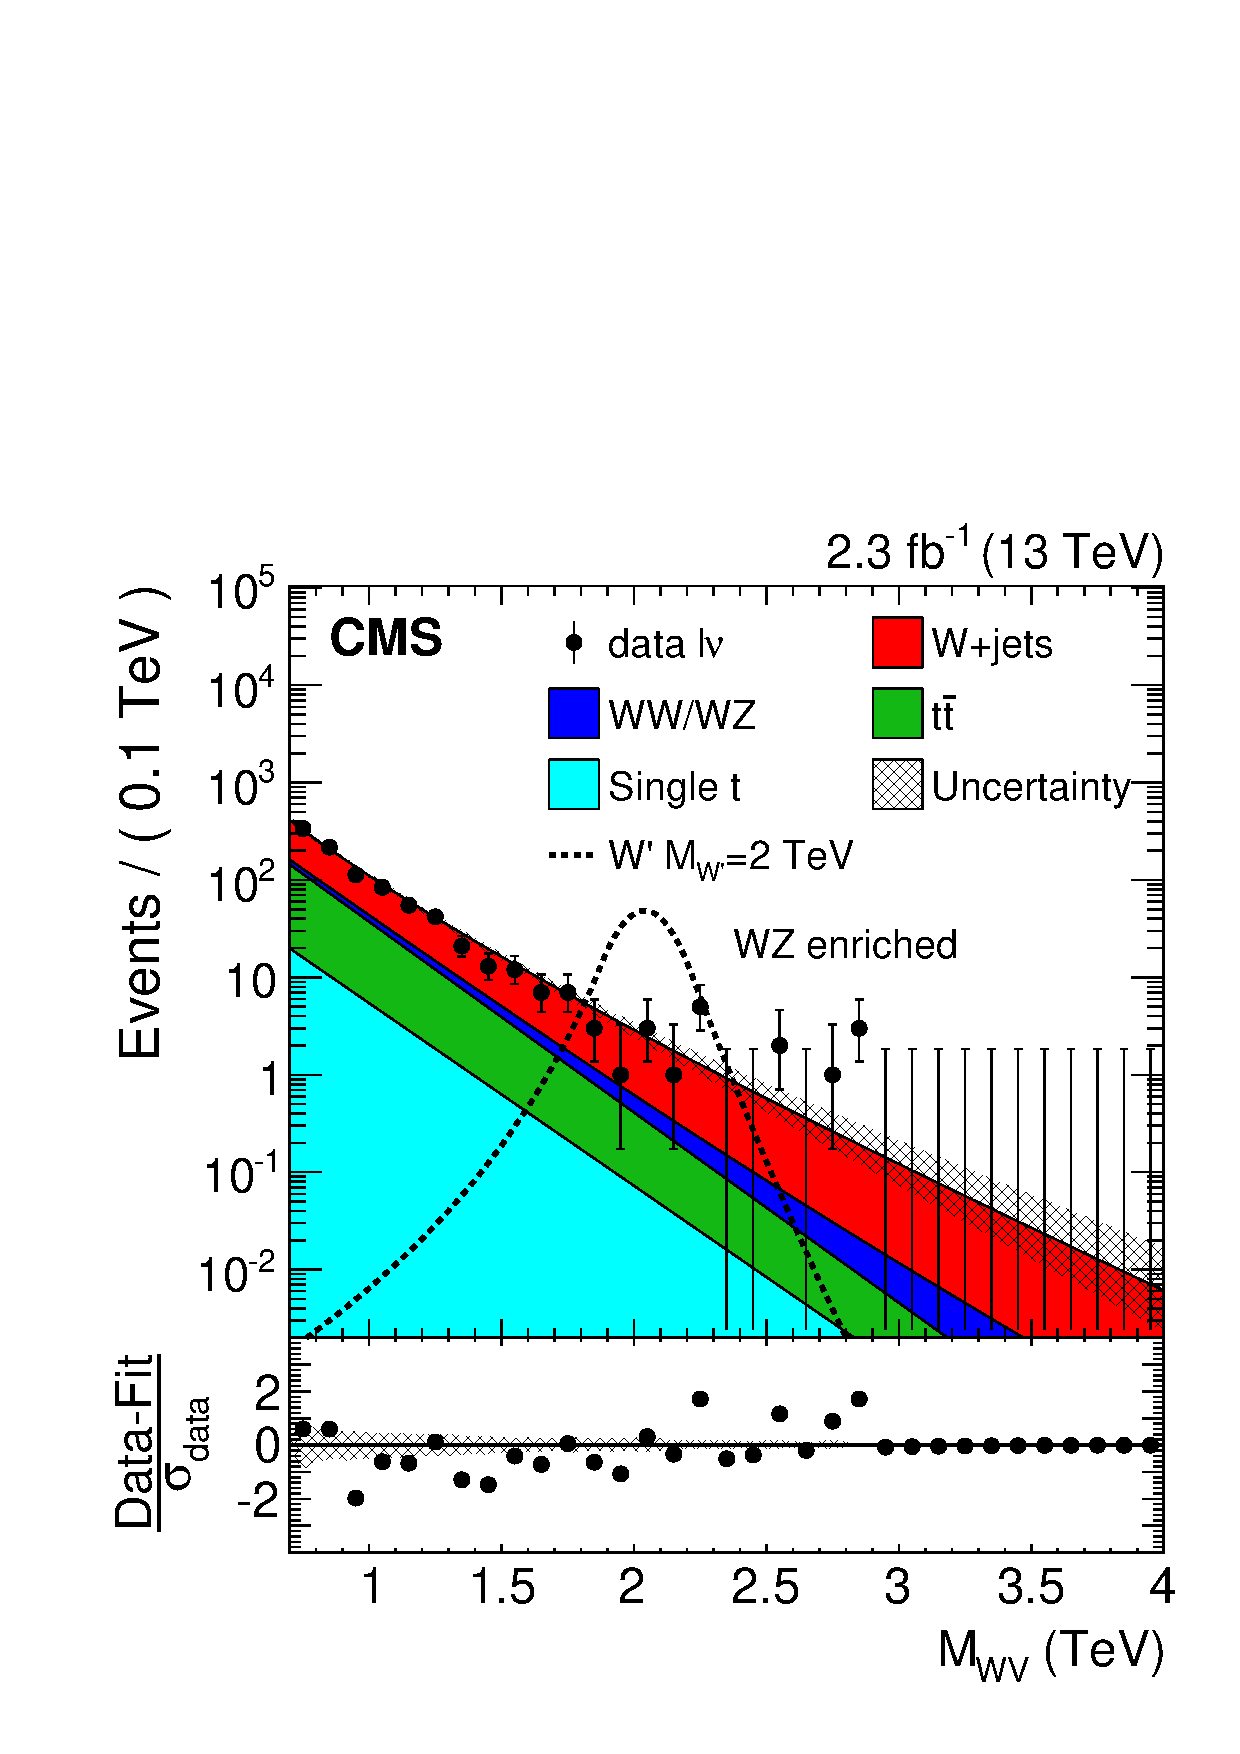
\includegraphics[width=0.45\textwidth]{\chten/HPZ_mlvj_fitting-em-check_workspace_for_limit__with_pull_log.pdf}}
\caption{%
%Final $\mVV$ distributions for data and expected backgrounds in the high-mass analysis for both the muon (left) and the electron (right) channels, WW-enriched (top) and WZ-enriched (bottom) signal regions.
Final $\mWV$ distributions for data and expected backgrounds obtained combining muon and electron channels in the WW-enriched (a) and WZ-enriched (b) signal regions.
In each plot the solid curve represents the background estimation provided by the $\alpha$ ratio method.
The hatched band includes both statistical and systematic uncertainties.
The data are shown as black points. At the bottom of each plot are the bin-by-bin fit residuals, ($N_\mathrm{data} - N_\mathrm{fit}$)/$\sigma_{\rm data}$, shown together with the uncertainty band of the fit normalized by the statistical uncertainty of data, $\sigma_{\rm data}$. The distributions for a bulk graviton and for a \Wpr signal are also shown with black dashed lines.}
\label{fig:mWV-final}
\end{figure}

%%%%%%%%%%%%%%%%%%%%%%%%%%%%%%%%%
\section{Cross section limits}
%%%%%%%%%%%%%%%%%%%%%%%%%%%%%%%%%

Since no excesses with significance larger than three standard deviations are observed, upper limits are set on the production cross section of the new resonance by combining all event categories.
The asymptotic approximation of the $\mathrm{CL}_s$ criterion described in Section~\ref{sec:stat} is followed.
The exclusion limits computed with this approach are found to agree with the results obtained using the modified frequentist prescription.
Systematic uncertainties are treated as nuisance parameters in the statistical interpretation using log-normal, and they are profiled following the frequentist convention as discussed in Section~\ref{sec:stat}.\\

Exclusion limits are set in the context of the bulk graviton model and of the HVT Models A and B, under the assumption of a natural width negligible compared to the experimental resolution.
Figure~\ref{fig:limitsAsympt-WV} shows the resulting 95\% CL expected and observed exclusion limits on the signal cross section as a function of the resonance mass for all signal hypotheses.
The limits are compared with the product of cross section and branching fraction ($\sigma\times\cal{B}$) to WW for a bulk graviton with $k/\bar{M}_\mathrm{Pl}$ = 0.5,
and with $\sigma\times\cal{B}$ for WZ and WW for spin-1 particles predicted by the HVT Models A and B.
In this context, a scenario is considered, where the $\Wpr$ and $\Zpr$ bosons are expected to be degenerate in mass (triplet hypothesis).
In addition, the statistical interpretation is provided in a scenario where only a charged ($\Wpr$) or a neutral ($\Zpr$) resonance is expected at a given mass (singlet hypothesis).

In the narrow-width bulk graviton model, the sensitivity of the search is not large enough to set mass limits, however, cross sections are excluded in the range 0.007--0.4 pb.
For HVT Model A (B), the data exclude singlet \Wpr resonances with masses $< 1.6$ (1.9)\TeV and \Zpr resonances with masses below $< 1.5$ (1.6)\TeV.
Under the triplet hypothesis, spin-1 resonances with masses $< 1.9$ and $< 2\TeV$ are excluded for HVT Models A and B, respectively.

These results supersede the ones obtained analyzing 8\TeV data, where the lower mass limit of 1.5\TeV for a $\Wpr$ in the context of the HVT model B is reached (Fig.~\ref{fig:limitsFullCLS-WH}).
However, the most stringent limits are obtained in the final combination of these results with other searches for heavy resonances decaying into diboson with 8 and 13\TeV data, as described in Chapter~\ref{ch:combination}.

\begin{figure}[!htb]
\centering
\subfigure[]{\label{fig:limitsAsympt-WV_a}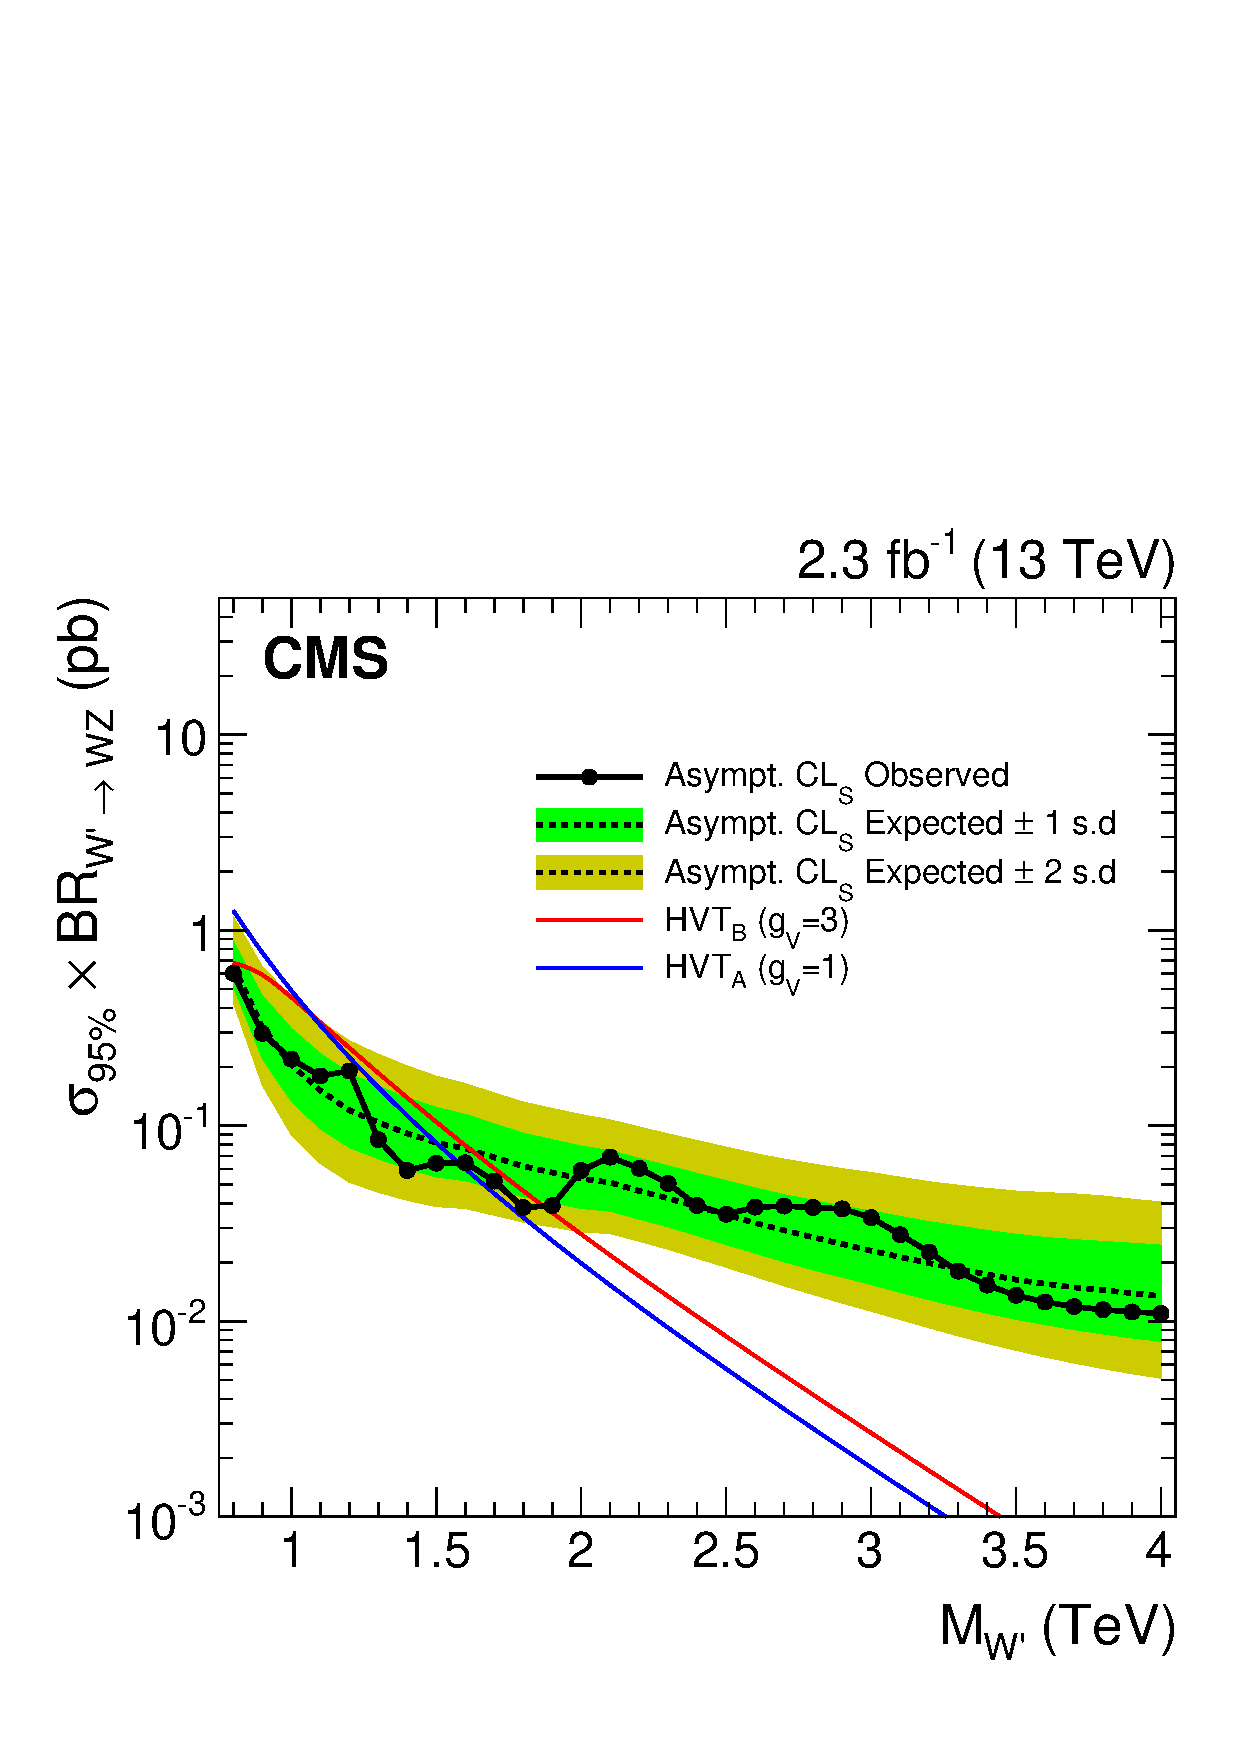
\includegraphics[width=0.45\textwidth]{\chten/EXOVVhvt_lvjwz13_UL_Asymptotic_log.pdf}}
\subfigure[]{\label{fig:limitsAsympt-WV_b}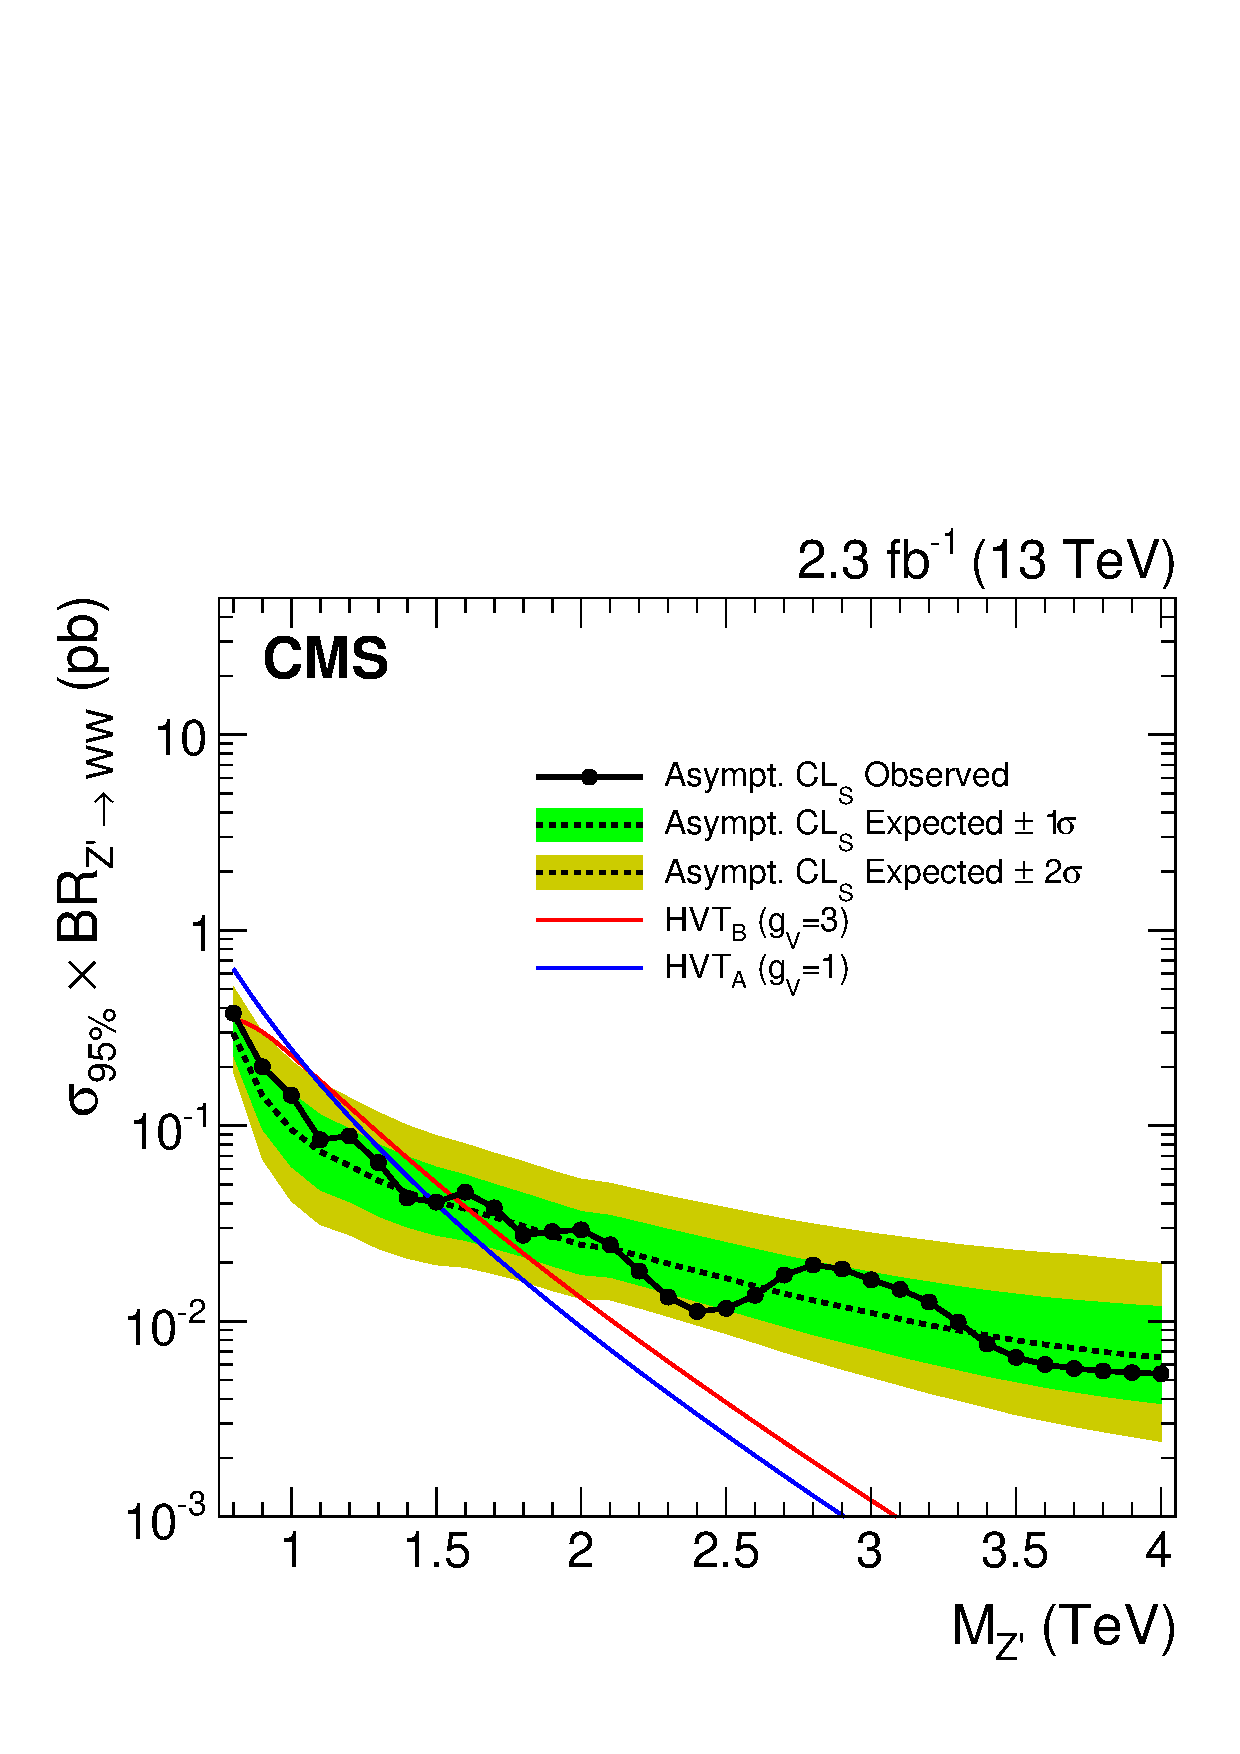
\includegraphics[width=0.45\textwidth]{\chten/EXOVVhvt_lvjww13_UL_Asymptotic_log.pdf}}
\subfigure[]{\label{fig:limitsAsympt-WV_c}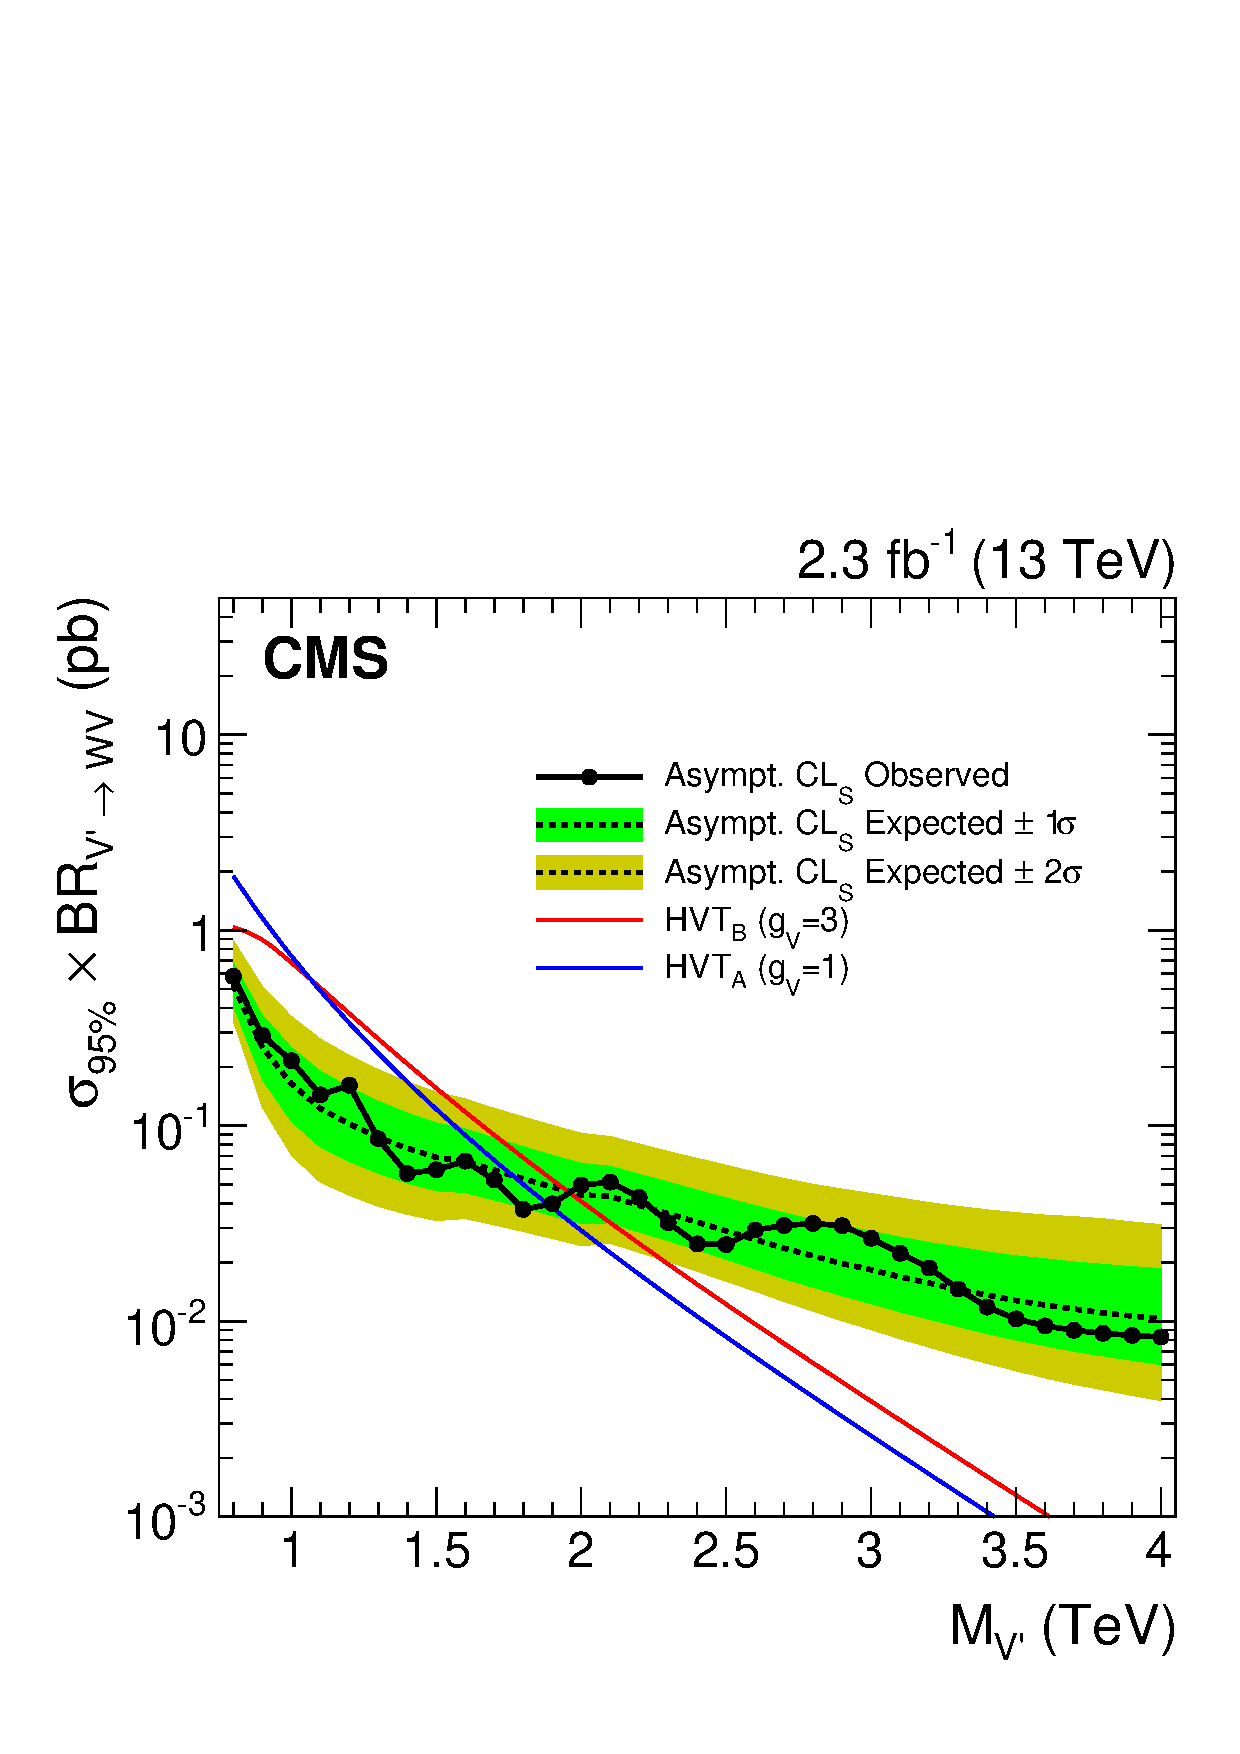
\includegraphics[width=0.45\textwidth]{\chten/EXOVVhvt_lvjwv13_UL_Asymptotic_log.pdf}}
\subfigure[]{\label{fig:limitsAsympt-WV_d}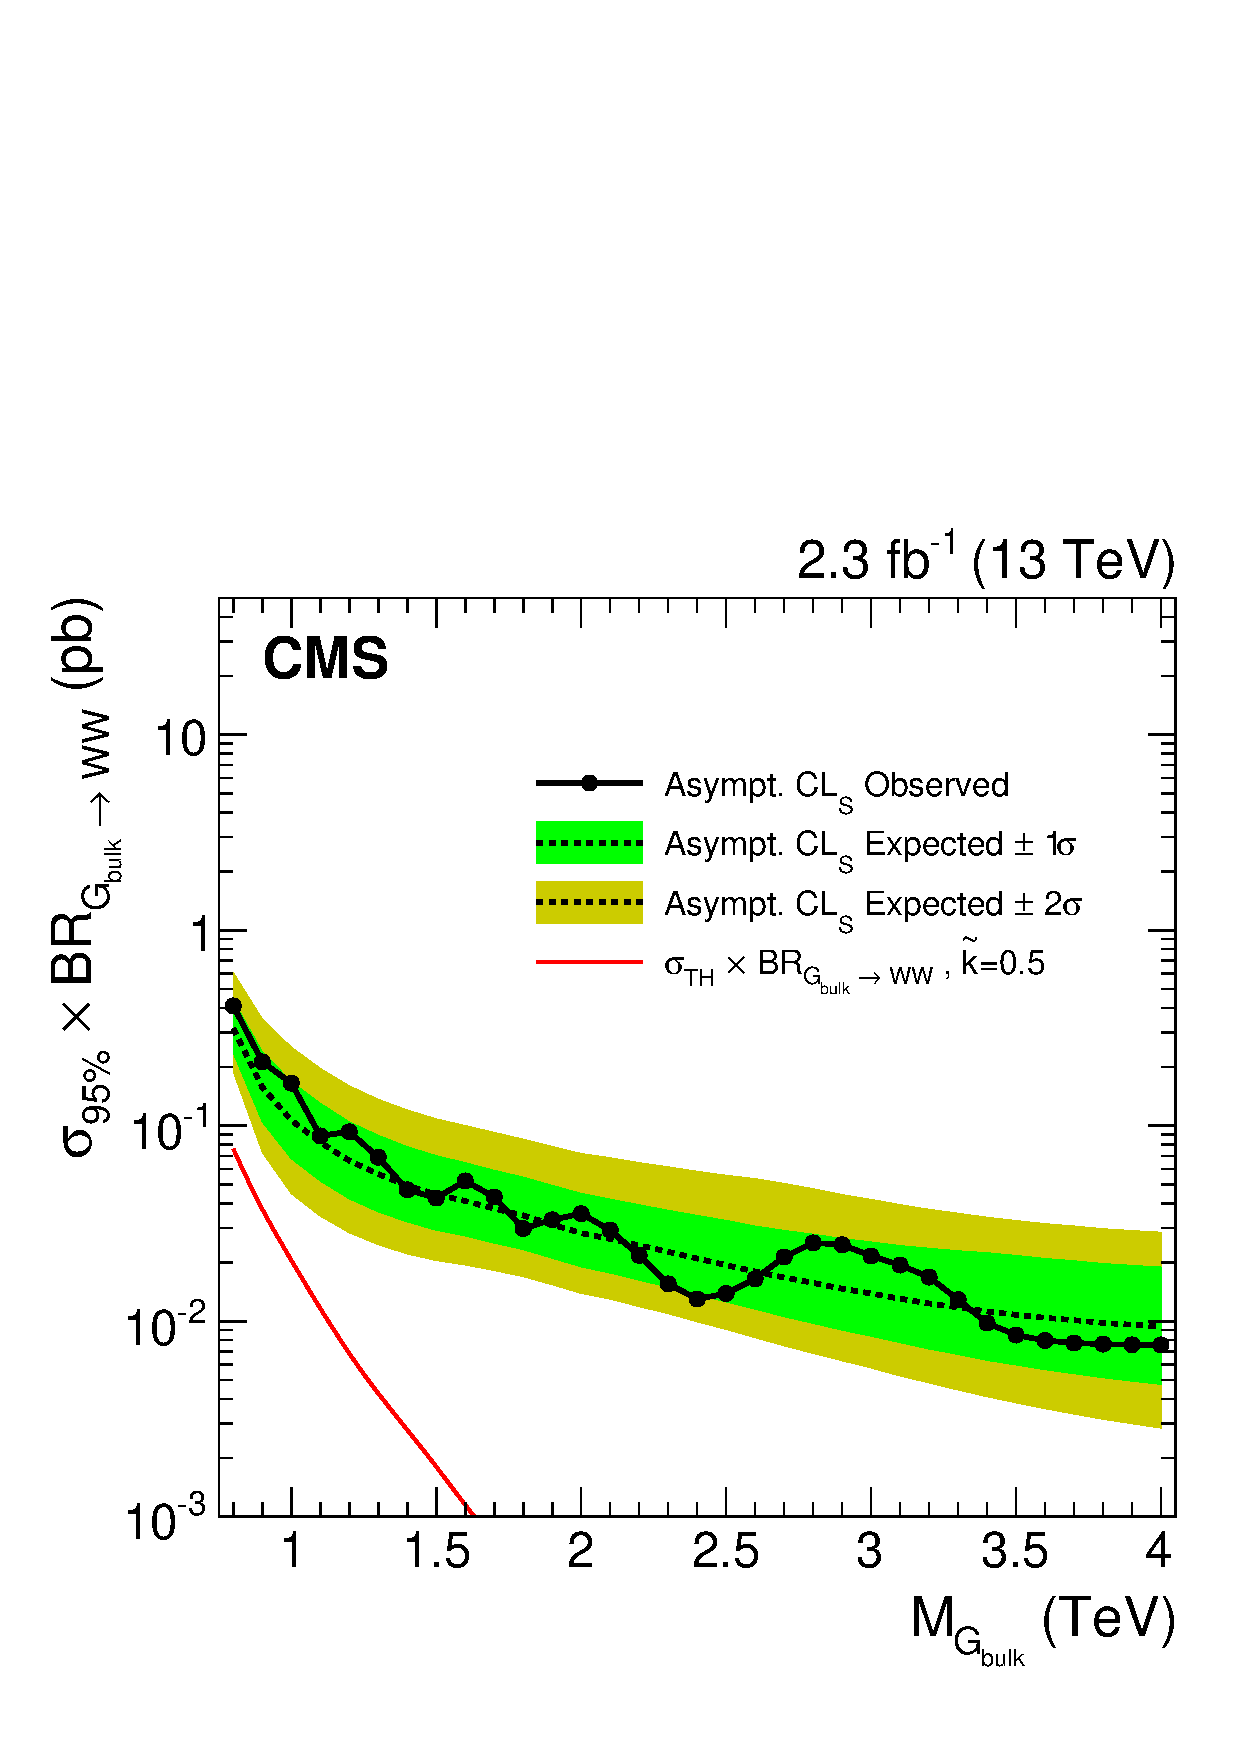
\includegraphics[width=0.45\textwidth]{\chten/EXOVVbulkg_xww13_UL_Asymptotic_log.pdf}}
\caption{Observed (black solid) and expected (black dashed) 95\% CL upper limits on the production of a narrow-width resonance decaying to a pair of vector bosons for different signal hypotheses.
In the upper plots, limits are set in the context of a spin-1 charged $\Wpr$ (a) and neutral $\Zpr$ (b) resonances, and compared with the prediction of the HVT Models A and B.
(c) Limits are set in the same model under the triplet hypothesis ($\Wpr$ and $\Zpr$). (d) Limits are set in the context of a bulk graviton with $k/\bar{M}_\mathrm{Pl}$ = 0.5 and compared with the prediction.
}
\label{fig:limitsAsympt-WV}
\end{figure}
